\documentclass[11pt]{article}
\usepackage[margin=1in]{geometry}
\usepackage{graphicx}
\usepackage{booktabs}
\usepackage{amsmath,amssymb}
\usepackage{microtype}
\usepackage{hyperref}
\usepackage{xcolor}
\usepackage{enumitem}
\usepackage[T1]{fontenc}
\usepackage[utf8]{inputenc}
\usepackage{float}
\usepackage{longtable}
\usepackage{tcolorbox}
\tcbuselibrary{breakable}
\usepackage{setspace}
\onehalfspacing

\graphicspath{{../results/figures/}}

\definecolor{boxblue}{RGB}{230,238,250}
\definecolor{boxyellow}{RGB}{255,246,220}
\definecolor{boxgreen}{RGB}{230,246,230}
\definecolor{boxred}{RGB}{253,232,232}
\definecolor{boxpurple}{RGB}{240,230,250}

\newtcolorbox{jargon}[1]{colback=boxblue,colframe=blue!55!black,
  title={Jargon unpacked: #1},fonttitle=\bfseries,breakable}
\newtcolorbox{whyblock}{colback=boxyellow,colframe=orange!60!black,
  title={Why we do this},fonttitle=\bfseries,breakable}
\newtcolorbox{resultbox}{colback=boxgreen,colframe=green!45!black,
  title={What this number means},fonttitle=\bfseries,breakable}
\newtcolorbox{pitfall}{colback=boxred,colframe=red!60!black,
  title={Pitfall / honest caveat},fonttitle=\bfseries,breakable}
\newtcolorbox{vnewbox}{colback=boxpurple,colframe=purple!55!black,
  title={New in v3},fonttitle=\bfseries,breakable}

\title{The ``Everything Explained'' Guide (v3)\\
\large{A newbie-friendly walkthrough of:\\
Dispersion, not displacement --- loss of alveolar epithelial\\
state coherence in lethal COVID-19}}
\author{Computational Systems Biology class project}
\date{\today}

\begin{document}
\maketitle

\begin{abstract}
\noindent This document explains the entire project from scratch. It assumes you have never touched single-cell RNA sequencing, never heard of diffusion pseudotime, and never dissected a lung. By the end you should be able to explain to anyone: (1) what the scientific question is; (2) what every technical term means; (3) where the data came from; (4) every computational step and what it computed; (5) what every figure, plot, and table shows; (6) how the conclusions were assembled; (7) what we are \emph{not} claiming and why; (8) the new donor-level analyses, portable state scores, and mechanistic decomposition added in v3.

Boxes are colour-coded:
\begin{itemize}
\item \textcolor{blue!55!black}{\textbf{Blue}} boxes unpack technical jargon.
\item \textcolor{orange!60!black}{\textbf{Yellow}} boxes say \emph{why} we do a step.
\item \textcolor{green!45!black}{\textbf{Green}} boxes interpret a specific number or plot.
\item \textcolor{red!60!black}{\textbf{Red}} boxes flag pitfalls and honest limitations.
\item \textcolor{purple!55!black}{\textbf{Purple}} boxes highlight what's new in v3.
\end{itemize}
\end{abstract}

\tableofcontents
\clearpage

% =========================================================================
\section{Part 1 --- The question in plain English}
% =========================================================================

Your lungs contain about 480 million microscopic air sacs called \emph{alveoli}. Their inner wall is a thin sheet of cells --- the \emph{alveolar epithelium} --- where oxygen crosses into your blood. In people who died of severe COVID-19, this sheet is visibly broken: cells are missing, abnormal cells appear, and new-looking cells are stuck mid-transformation.

The specific question of this project is:

\begin{quote}
\textbf{When the alveolar epithelium fails in lethal COVID-19, does it fail in a \emph{coordinated} way (every sick cell moves toward one damaged state), or in a \emph{dispersed} way (cells scatter in many different directions at once)?}
\end{quote}

These two possibilities look geometrically different and predict different things:

\begin{itemize}
\item If it's \textbf{coordinated displacement}: the COVID cells as a group sit at a clearly different spot from healthy cells. Their group average (centroid) has shifted.
\item If it's \textbf{heterogeneous dispersion}: the COVID cells' group average may not move much, but the \emph{spread} of COVID cells --- how far each one sits from its own group center --- is much larger than in healthy cells.
\end{itemize}

We call the dispersed pattern \emph{loss of state coherence}: the tissue loses its ability to keep every cell in a tight, healthy identity. Cells drift apart from one another along many axes of gene expression at once, without converging on any single ``damaged'' state.

\begin{jargon}{what ``state coherence'' means here}
In a healthy organ, cells of a given type (e.g.\ every AT2 cell) look very similar to each other in their gene expression. That uniformity reflects a working regulatory network that pins cells into a shared identity. Stress or damage can weaken this pinning, so cells drift apart. The \emph{loss of uniformity} itself is the signature of coherence loss --- even if no single ``damaged'' state is reached.
\end{jargon}

\begin{whyblock}
We measure \emph{two different things} on purpose. Measuring only the group average (centroid displacement) would miss the dispersed pattern. Measuring only the spread (dispersion) would miss the coordinated pattern. We commit \emph{in advance} to declaring which outcome supports which hypothesis. This is how you do honest hypothesis testing.
\end{whyblock}

\paragraph{What this project is NOT.}
We are \textbf{not} discovering new biology about COVID-19 lungs. Melms et al.\ (2021), Delorey et al.\ (2021), and others already described alveolar injury, transitional cell accumulation, and donor heterogeneity. Our contribution is \textbf{methodological}:
\begin{enumerate}
\item Pre-register multiple geometric tests that distinguish different mechanisms.
\item Stress-test conclusions with ten systematic ablations.
\item Audit with an independent 618-donor out-of-cohort replication.
\item Add donor-level modeling to address the ``$n = 27$ donors, not 22{,}128 cells'' problem.
\item Develop portable, continuous state scores that transfer across cohorts.
\item Report honestly which findings survive and which don't.
\end{enumerate}


% =========================================================================
\section{Part 2 --- Biology in plain terms}
% =========================================================================

\subsection{The alveolar epithelium: a two-cell sheet}

Two major epithelial cell types line each alveolus:

\begin{description}[style=nextline]
\item[AT1 cells (alveolar type 1)] Very flat, very thin. They cover $\approx$95\% of the alveolar surface. Their job is \emph{gas exchange}: oxygen in, carbon dioxide out. They do not divide.
\item[AT2 cells (alveolar type 2)] Cube-shaped, smaller surface coverage. Two jobs: (i) secrete \emph{surfactant}, a soapy fluid that stops alveoli collapsing when you exhale; (ii) serve as local \emph{stem cells}: when AT1 cells die, AT2 cells divide and transform into new AT1 cells through a temporary, fragile state called the \emph{transitional} or \emph{DATP} state.
\end{description}

\begin{jargon}{DATP / transitional cell}
A cell that used to be AT2 and is in the process of becoming AT1. It has a characteristic gene signature: strong expression of KRT8, CLDN4, SFN; weakened AT2 markers; partial AT1 markers. In healthy adult lungs these cells are rare. In acute lung injury they accumulate --- cells get stuck mid-transition and never finish becoming AT1.
\end{jargon}

\subsection{Why COVID-19 hurts this particular sheet}

SARS-CoV-2 enters AT2 cells through the ACE2 receptor. This is particularly bad because AT2 cells are \emph{both} the surfactant-producing cells (so when they fail, alveoli collapse) \emph{and} the local stem cells (so when they fail, AT1 cells can't be replaced). On top of direct viral damage, the body's inflammatory response inflicts collateral damage. In lethal cases, autopsies show \emph{diffuse alveolar damage}: holes in the AT1 sheet, edema, and abnormal cells caught mid-transition.

\begin{jargon}{snRNA-seq (single-nucleus RNA sequencing)}
A way to measure which genes are active in thousands of individual cells simultaneously. In frozen post-mortem tissue, you can't isolate whole cells (they fall apart), so you isolate individual cell \emph{nuclei} instead. Each nucleus's messenger RNA is barcoded and sequenced, giving you a counts-per-gene vector per nucleus. People use this for autopsy tissue where whole cells cannot be recovered.
\end{jargon}

\subsection{Key vocabulary}

\begin{description}[style=nextline,leftmargin=0pt]
\item[Gene expression] The amount of messenger RNA produced from a gene in a cell. Measured as a count (UMIs).
\item[Expression vector] A long list of numbers, one per gene, describing each cell's activity.
\item[Matrix X] All expression vectors stacked: rows = cells, columns = genes. The fundamental data object.
\item[UMI] Unique Molecular Identifier. A short random DNA tag added to each RNA molecule before amplification, so we count distinct molecules rather than PCR duplicates.
\item[HVG (Highly Variable Gene)] A gene that varies a lot between cells. These carry most of the biological signal; the rest are mostly noise.
\item[PCA (Principal Component Analysis)] Compresses each cell's expression from $\sim$20{,}000 genes down to 50 numbers that preserve most of the variance.
\item[UMAP] A non-linear algorithm that places each cell on a 2-D map for visualization. Cells near each other had similar expression. \emph{For seeing, not for measuring.}
\item[Diffusion map / DPT] A mathematically principled way to order cells along a continuous biological process. Root it at a ``starting'' cell; cells further along get larger pseudotime values.
\item[Gene program] A hand-curated list of genes reflecting one biological process (e.g.\ interferon response). Score each cell by averaging the expression of that program's genes.
\item[Batch effect] Systematic technical differences between samples (different donors, different days) that aren't biology.
\item[Harmony] An algorithm that adjusts PCA coordinates to remove batch effects while preserving real biological structure.
\item[Ablation] Systematically changing one piece of the pipeline to test if the conclusion still holds.
\item[Pseudobulk] Aggregating single-cell data to one value per donor (e.g., taking the median across all cells from one donor). This lets you use the donor as the statistical unit instead of the cell.
\item[Levene's test] A statistical test that asks whether two groups have different \emph{spread} (variance), regardless of their means.
\item[Mann--Whitney U test] A non-parametric test that asks whether values in one group tend to be larger than in another.
\item[Bootstrap] Resampling your data with replacement many times to estimate the uncertainty (confidence interval) of a statistic.
\item[OLS (Ordinary Least Squares)] The simplest form of linear regression: fit a straight line through data points and report the slope.
\end{description}


% =========================================================================
\section{Part 3 --- Where the data came from}
% =========================================================================

\subsection{Primary cohort: SCP1219 (Melms 2021)}

A publicly released single-nucleus RNA-seq atlas of post-mortem lung tissue from patients who died of COVID-19, plus healthy organ donors as controls.

\begin{itemize}
\item \textbf{Donors}: 20 COVID-19 patients (post-mortem) + 7 healthy organ donors = 27 total.
\item \textbf{Total nuclei sequenced}: 116{,}313.
\item \textbf{Assay}: 10x Genomics 3' v3 single-nucleus RNA-seq.
\item \textbf{After subsetting to alveolar epithelium}: 22{,}128 cells: AT1 (9{,}608), AT2 (11{,}341), ECM-high/transitional (1{,}179).
\item \textbf{Per-donor cell counts}: range 62 to 2{,}850. Ten donors contribute fewer than 300 cells each.
\end{itemize}

\begin{pitfall}
The true sample size is 27 donors (7 vs 20), \textbf{not} 22{,}128 cells. Cells from the same donor are not independent observations. Every primary statistical claim must hold at the donor level, not just the cell level. This is why v3 adds explicit donor-level modeling.
\end{pitfall}

The data is stored as an \texttt{.h5ad} file (AnnData format), which bundles: \texttt{adata.X} (the counts matrix), \texttt{adata.obs} (per-cell metadata: condition, donor ID, cell type), and \texttt{adata.var} (per-gene metadata).

\subsection{Replication cohort: cellxgene census}

For independent replication, we pulled data from the cellxgene census (CZI's curated federation of single-cell datasets):

\begin{itemize}
\item 89{,}736 alveolar AT1/AT2 cells after per-donor subsampling (cap 200 cells/donor).
\item 618 donors (43 COVID-19, 575 normal) from 35 datasets.
\item The primary cohort (SCP1219) was \textbf{excluded by dataset ID} --- we cannot accidentally replicate on the same data.
\item Only 84 genes downloaded (the genes in our 8 scoring programs + canonical markers).
\end{itemize}

\begin{pitfall}
The replication is not full-transcriptome: 84 genes is enough to score programs and compute dispersion on those scores, but too narrow to build a new manifold or run diffusion pseudotime from scratch. This is an honest limitation.
\end{pitfall}


% =========================================================================
\section{Part 4 --- The computational pipeline, step by step}
% =========================================================================

All code is in \texttt{src/} with orchestration in \texttt{scripts/}. Every parameter is in \texttt{config.yaml}. Software: Python 3.12.3, Scanpy 1.12.1, AnnData 0.12.10, harmonypy 0.2.0, palantir 1.4.4. Random seed fixed to 42.

\subsection{Step 1 --- Quality control (QC)}

Each nucleus has a total UMI count and a percentage of reads from mitochondrial genes. We filter out junk:

\begin{itemize}
\item $\geq$200 genes per cell (remove empty droplets)
\item $\leq$8{,}000 genes per cell (remove doublets)
\item $\leq$20\% mitochondrial reads (remove dying cells)
\item Drop genes detected in $<$10 cells
\end{itemize}

\begin{whyblock}
QC is the most underrated step. Let junk cells through and every downstream statistic is contaminated. Be too aggressive and you delete real biology.
\end{whyblock}

\subsection{Step 2 --- Subset to alveolar epithelium}

The atlas has pre-computed cell-type labels. We keep AT1, AT2, and ECM-high epithelial (the transitional state). We validate labels by checking that canonical marker genes are actually higher in the right cells: SFTPC in AT2, AGER in AT1, KRT8/CLDN4 in transitional.

\subsection{Step 3 --- Normalization and log-transformation}

\begin{enumerate}
\item \textbf{Normalize}: rescale every cell's expression vector to sum to 10{,}000. This removes depth differences between cells.
\item \textbf{Log-transform}: take $\log(1+x)$ of every count. Compresses dynamic range and makes distributions closer to normal.
\item \textbf{Save raw}: store the full log-normalized matrix in \texttt{adata.raw} for later gene-program scoring.
\end{enumerate}

\subsection{Step 4 --- Highly variable gene selection}

Pick the 3{,}000 most biologically variable genes (Seurat v3 method). Most of the $\sim$20{,}000 genes are too noisy to carry signal.

\subsection{Step 5 --- Scale + PCA}

Scale each gene to mean 0, variance 1 (clipped at 10). Run PCA and keep 50 components. After this, every cell is a 50-number vector stored in \texttt{adata.obsm["X\_pca"]}.

\begin{jargon}{why 50 PCs?}
5 is too few (you lose real biological axes). 500 starts including noise. 50 is standard for heterogeneous human tissue and our conclusions don't change with 30 or 100 (tested in ablation).
\end{jargon}

\subsection{Step 6 --- Batch correction with Harmony}

Harmony repeatedly soft-clusters the PCA space and shifts each cluster so that donors are mixed rather than separated. Output: \texttt{X\_pca\_harmony}, a 50-dim matrix with donor structure reduced.

\begin{pitfall}
In v1 of this paper there was a \emph{silent orientation bug} in our Harmony wrapper. The old CPU backend returned the corrected matrix as (PCs, cells); the new PyTorch backend returns (cells, PCs). We were always transposing, which was right for the old backend and wrong for the new one. The fix was a one-line orientation check. Post-fix, Harmony \emph{strengthens} the pseudotime shift from $+0.048$ to $+0.125$ (2.6$\times$). This is the most important methodological lesson in this paper: ``batch correction didn't help'' can mean ``my wrapper is broken.''
\end{pitfall}

\subsection{Step 7 --- Neighbor graph, UMAP, diffusion map}

\begin{enumerate}
\item \textbf{$k$-NN graph}: connect each cell to its 15 nearest neighbors in PCA space.
\item \textbf{UMAP}: 2-D layout for figures. \emph{Visualization only --- never used for statistics.}
\item \textbf{Diffusion map}: a different 15-D coordinate system designed so that ``random-walk distance'' is easy to compute. This is the basis for pseudotime.
\end{enumerate}

\subsection{Step 8 --- Diffusion pseudotime (DPT)}

Pick a root cell (the cell closest to the centroid of all healthy AT2 cells in diffusion map space). Compute diffusion distance from that root for every cell. Normalize to $[0,1]$.

\begin{jargon}{what pseudotime IS and IS NOT}
Pseudotime is an \emph{ordering}, not a clock. A cell with pseudotime 0.8 is ``further along the manifold'' from the root than a cell with 0.3, but this says nothing about elapsed hours. It reflects the geometry of gene-expression similarity.
\end{jargon}

\subsection{Step 9 --- Gene program scoring}

Eight curated gene programs, each a list of genes reflecting one biological process:

\begin{itemize}
\item AT2 identity (9 genes: SFTPC, SFTPA1, SFTPA2, ABCA3, LAMP3, SLC34A2, NAPSA, PGC, LPCAT1)
\item AT1 identity (8 genes: AGER, PDPN, HOPX, CLIC5, CAV1, EMP2, AKAP5, RTKN2)
\item Interferon response (13 genes)
\item NF-$\kappa$B inflammatory (12 genes)
\item Oxidative stress (12 genes)
\item AT2-to-AT1 differentiation (8 genes: KRT8, CLDN4, SFN, KRT18, LGALS3, HOPX, AGER, PDPN)
\item Apoptosis (13 genes)
\item Senescence (10 genes)
\end{itemize}

Scoring uses scanpy's \texttt{score\_genes}: for each program and each cell, compute mean expression of program genes minus mean expression of a matched random background set. This background subtraction is essential --- without it, cells with overall higher expression would score higher on every program.

\subsection{Step 10 --- The three pre-registered statistical tests}

\paragraph{(a) Centroid displacement (one-sided Mann--Whitney $U$).}
Compute each cell's Euclidean distance to the healthy centroid in 50-D PCA space. Test whether COVID cells sit \emph{further} from the healthy centroid than healthy cells do.

\paragraph{(b) Dispersion (Levene's test).}
Compute each cell's distance to \emph{its own group's} centroid. Test whether the \emph{variance} of these within-group distances differs between COVID and Healthy.

\paragraph{(c) Pseudotime enrichment (1{,}000-permutation test).}
Shuffle condition labels 1{,}000 times, recompute median pseudotime difference each time, and see how extreme the real difference is.

\begin{resultbox}
All three tests were decided \emph{before} looking at the data, including which direction counts as ``supports the hypothesis.'' A failing test is informative --- it tells you which mechanism is wrong.
\end{resultbox}


% =========================================================================
\section{Part 5 --- Results: what the numbers actually say}
% =========================================================================

\subsection{Result 1 --- Centroid displacement FAILS}

\begin{resultbox}
\textbf{One-sided Mann--Whitney $U$}: $p = 1.0$. Rank-biserial $r = 0.14$ pointing \emph{opposite} to the hypothesized direction. COVID cells were actually \emph{closer} to the healthy centroid (median distance 10.68) than healthy cells were to their own centroid (11.56).
\end{resultbox}

This is not a failure of the study --- it's a positive finding. It rules out the simpler model where all COVID cells shift coherently toward one damaged phenotype. Some COVID cells stay near homeostatic identity while others scatter to distant positions. A mean-displacement test averages over both subpopulations and sees nothing.

\subsection{Result 2 --- Within-group dispersion SUCCEEDS (the main finding)}

\begin{resultbox}
\textbf{Levene's test}: statistic = 276.5, $p < 10^{-30}$. Within-group distance-to-centroid variance: COVID 33.28 vs.\ Healthy 14.58 (ratio 2.3$\times$). COVID cells occupy a 2.3-fold broader region of gene-expression space.
\end{resultbox}

This is the strongest signal in the entire study. It means COVID-19 cells don't converge on one damaged state --- they scatter across many partially overlapping injury states. We call this \emph{dispersion-dominated loss of state coherence}.

\begin{figure}[H]\centering
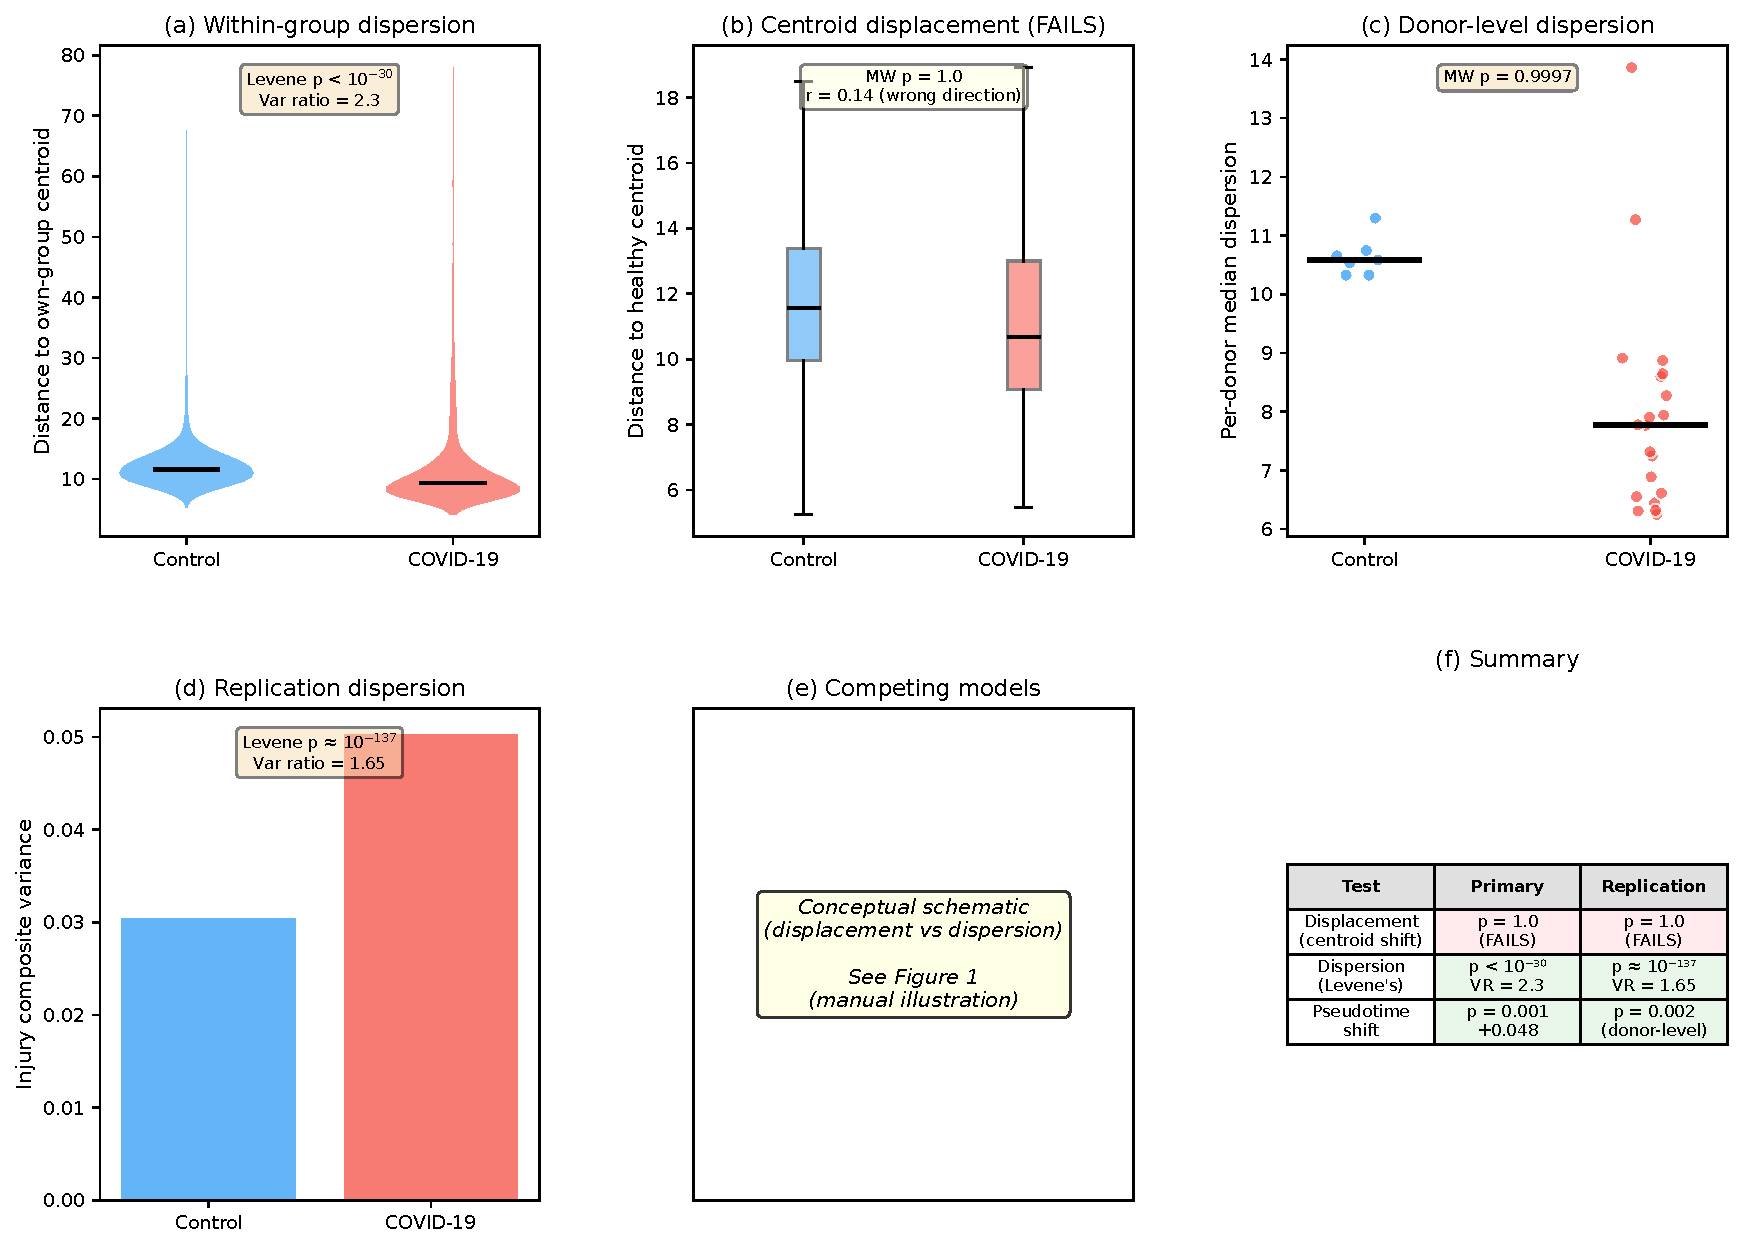
\includegraphics[width=\textwidth]{fig3_dispersion_centerpiece.pdf}
\caption{The dispersion centerpiece figure. Panel (a): within-group distance distributions. Panel (b): displacement test. Panel (c): donor-level dispersion. Panel (d): replication. Panel (e): summary statistics.}
\end{figure}

\subsection{Result 3 --- Pseudotime shift SUCCEEDS}

\begin{resultbox}
\textbf{Median pseudotime}: COVID 0.111 vs.\ Healthy 0.063. Difference $= +0.048$ ($\approx$5\% of the $[0,1]$ range). Permutation $p = 0.001$. Leave-one-donor-out: direction preserved in 27/27 iterations.
\end{resultbox}

The shift is modest but statistically robust. It means COVID cells are enriched at higher positions along the injury axis --- further from healthy AT2 identity. The shift is amplified 2.6$\times$ under Harmony batch correction, which is strong evidence it's real biology, not a batch artifact.

\begin{figure}[H]\centering
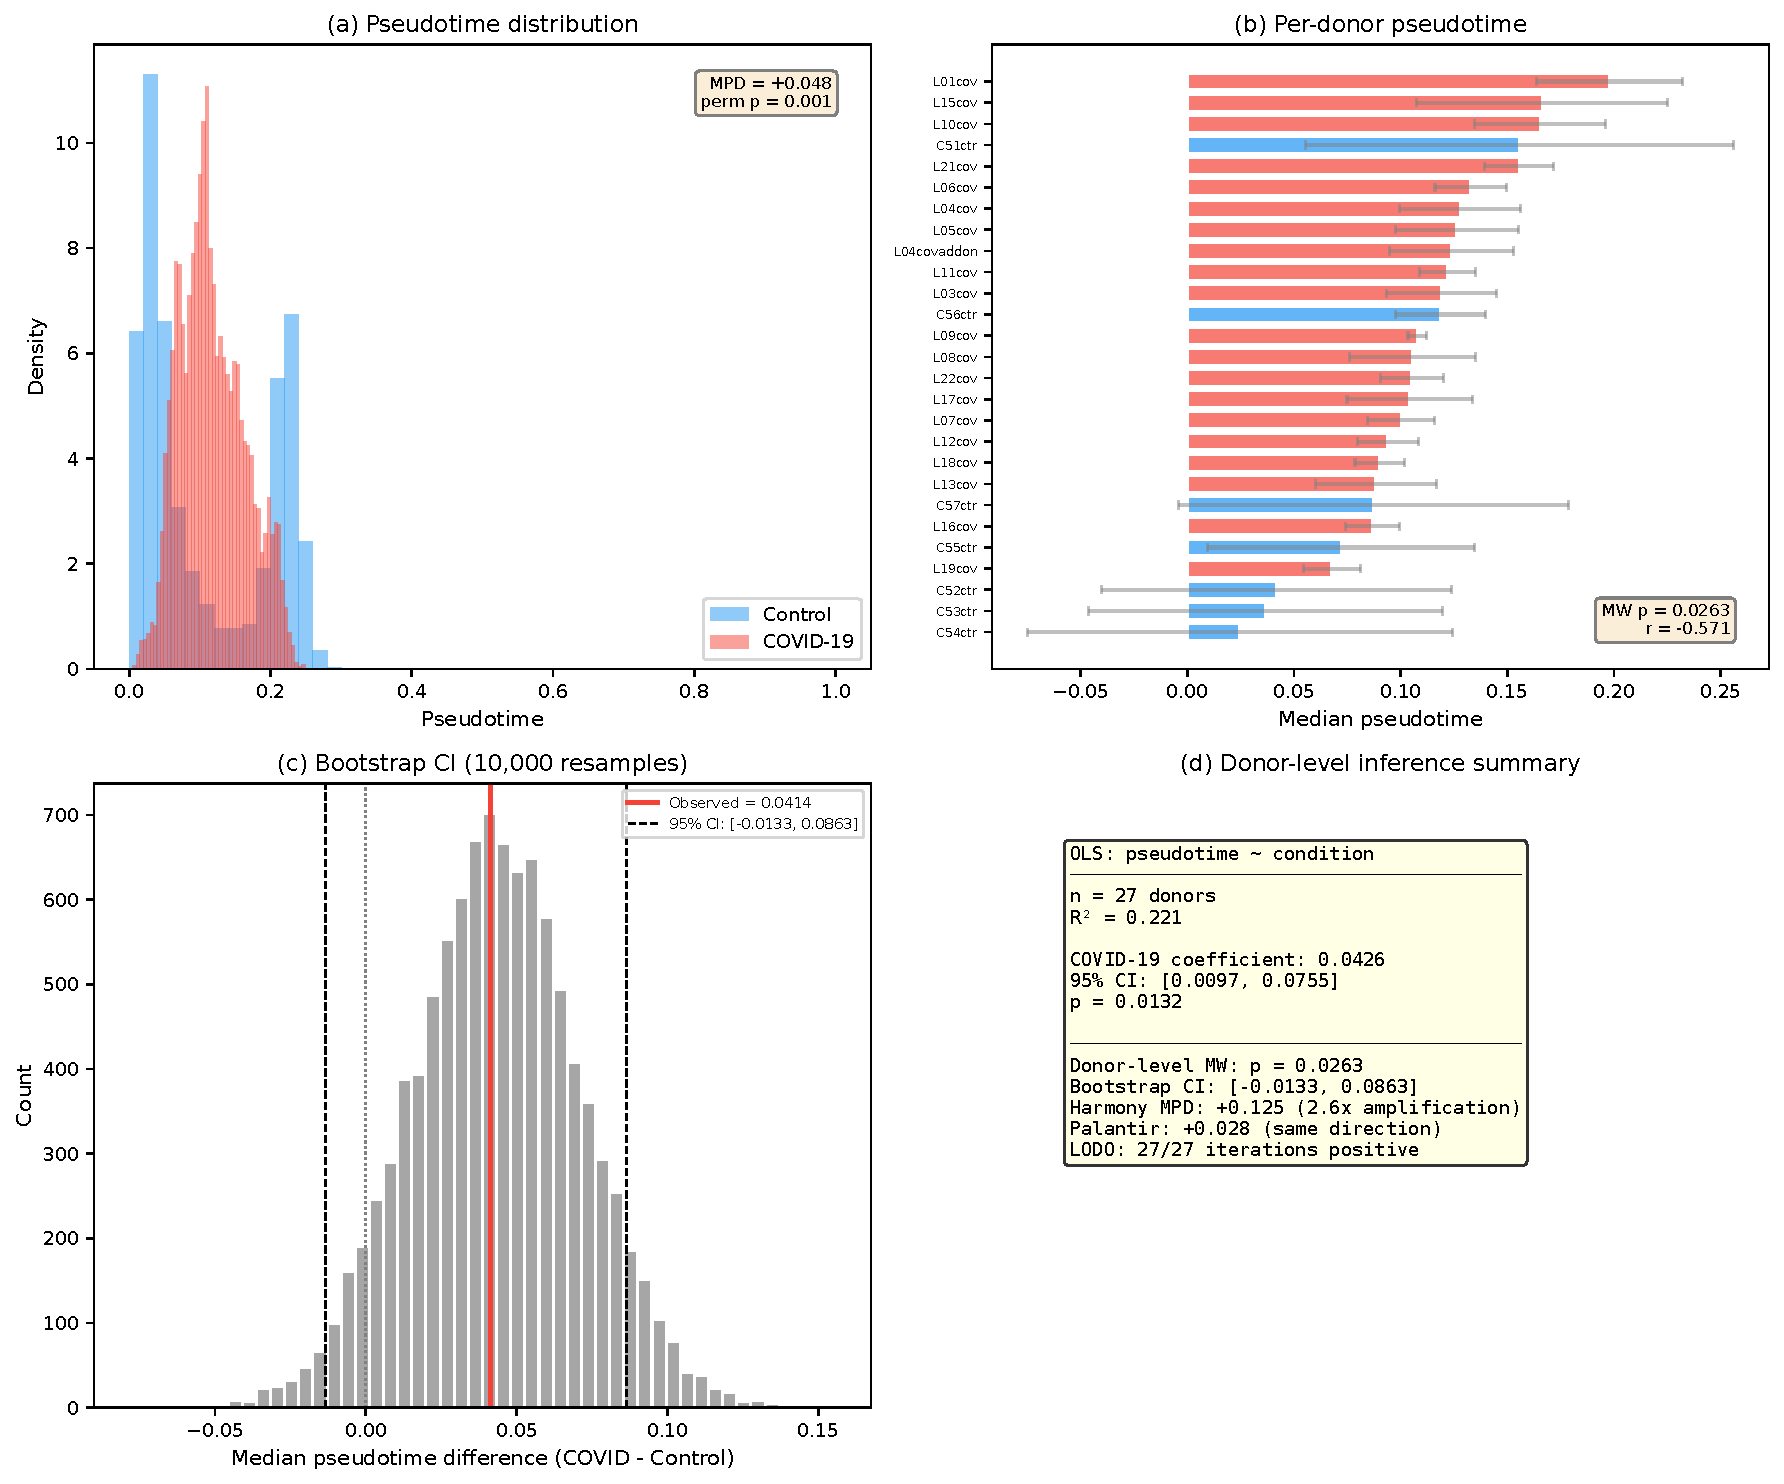
\includegraphics[width=\textwidth]{fig4_donor_pseudotime.pdf}
\caption{Donor-level pseudotime analysis. Per-donor median pseudotime, bootstrap CI, and OLS model.}
\end{figure}

\subsection{Result 4 --- Transitional cells enriched (primary atlas only)}

The ECM-high transitional population was enriched 3.1-fold in COVID-19 (8.5\% vs 2.7\%; $\chi^2$ $p < 10^{-30}$). These are cells stuck mid-transition from AT2 to AT1, consistent with damage-associated transient progenitors (DATPs) described in mouse injury models.

\begin{pitfall}
This enrichment does NOT replicate cross-cohort. In the replication cohort, the KRT8$^+$/CLDN4$^+$ threshold actually gives the \emph{opposite} result (COVID 22.9\% vs Normal 47.6\%). Marker-threshold cell-state definitions are not portable across studies with different protocols and normalization.
\end{pitfall}


% =========================================================================
\section{Part 6 --- The ten ablations (stress tests)}
% =========================================================================

An ablation means: ``change one pipeline choice, redo the tests, see what breaks.'' The goal is not to find the ``right'' answer but to learn which choices are load-bearing.

\begin{description}[style=nextline]
\item[Ablation 1: AT2-only] Drop AT1 and transitional cells. \emph{Sign flip on displacement --- the AT1 side matters.}
\item[Ablation 2: Alternative embeddings] Use UMAP/diffmap variants. \emph{Pseudotime shift and dispersion persist.}
\item[Ablation 3: Harmony vs uncorrected] Post-bug-fix, Harmony strengthens the shift 2.6$\times$ without changing dispersion.
\item[Ablation 4: Drop apoptosis genes] Remove apoptosis genes from manifold construction. \emph{Signal is not driven by an ``apoptosis axis.''}
\item[Ablation 5: Alternative roots] Try 4 different pseudotime roots. \emph{Direction stable for 3 of 4; COVID-extreme root inverts, as expected.}
\item[Ablation 6: Broader epithelial] Include airway cells. \emph{Pseudotime shift abolished --- confirms the signal is alveolar-specific.}
\item[Ablation 7: Leave-one-donor-out] Drop one donor at a time (27 iterations). \emph{Direction preserved 27/27 times. No single donor drives the result.}
\item[Ablation 8: Alternative programs] Swap gene lists. \emph{Curated-only: ordering preserved ($\rho = 1.0$). MSigDB-only: ordering inverts ($\rho = -0.80$). Fine ordering is fragile.}
\item[Ablation 9: Palantir] Different trajectory algorithm. \emph{Direction preserved, magnitude +0.028.}
\item[Ablation 10: Permutation] Shuffle labels 1{,}000 times. \emph{$p = 0.001$.}
\end{description}

\begin{figure}[H]\centering
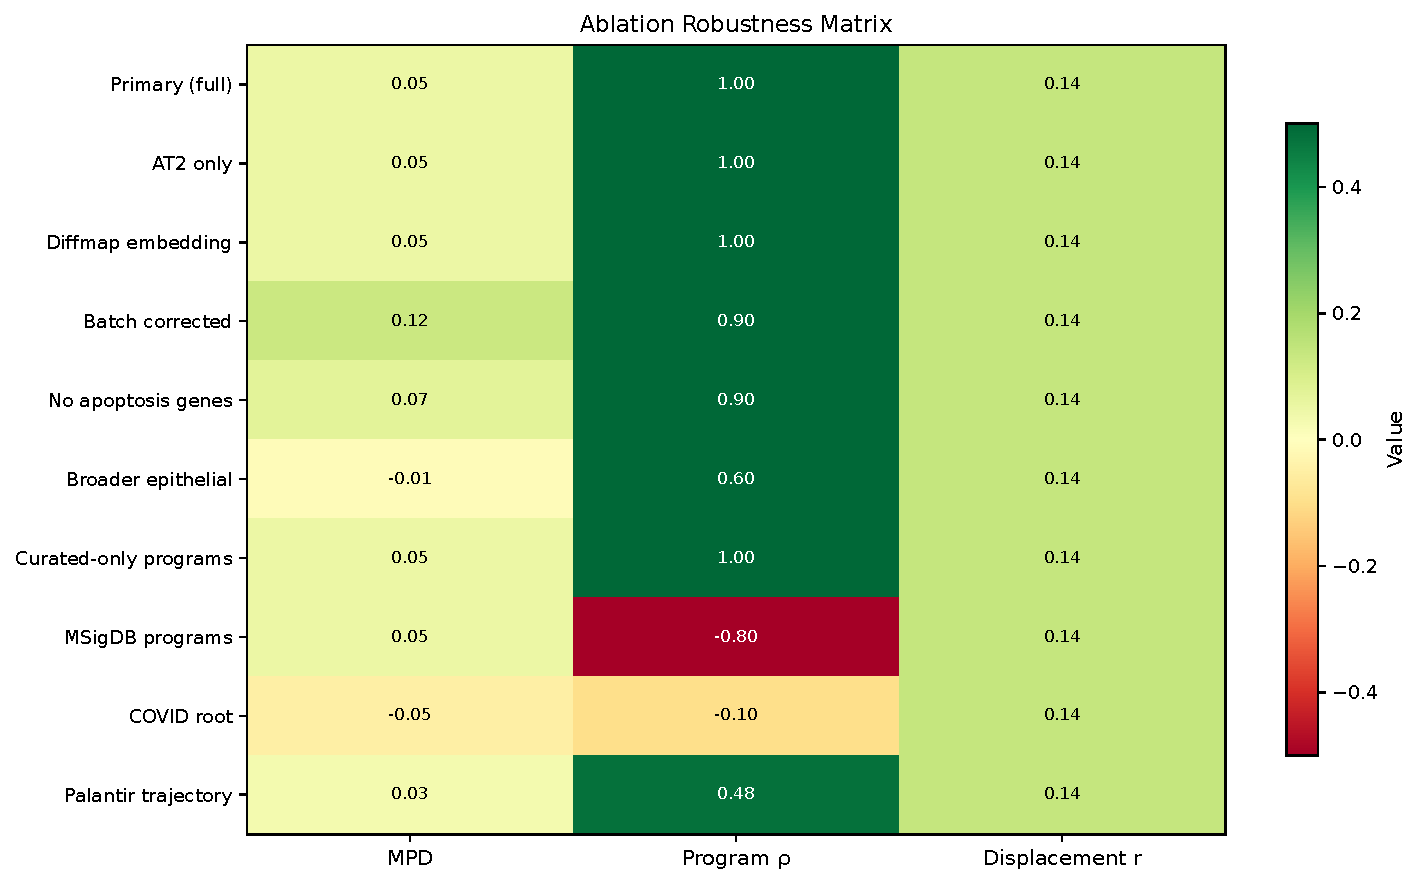
\includegraphics[width=\textwidth]{fig6_ablation_matrix.pdf}
\caption{Ablation robustness matrix. Rows: ablations. Columns: three metrics. Green = robust; red = fragile.}
\end{figure}

\begin{resultbox}
\textbf{Bottom line}: Dispersion and pseudotime direction are robust across all ablations. Fine-grained program ordering is fragile (it depends on which gene lists you use). The centroid-displacement failure is robust --- it never becomes significant in the pre-specified direction.
\end{resultbox}


% =========================================================================
\section{Part 7 --- Independent replication}
% =========================================================================

\subsection{What ``replication'' means here}

Did the same biological signature show up in completely different data that we never used when building the analysis? If yes, the finding is not an artifact of one cohort's protocol or donor mix.

\subsection{What replicated}

\begin{resultbox}
\textbf{Dispersion}: Levene statistic 626.2, $p \approx 10^{-137}$, variance ratio 1.65$\times$ (COVID/Normal). Across 35 independent datasets and 618 donors. \textbf{This is the most portable finding.}
\end{resultbox}

\begin{resultbox}
\textbf{Donor-level pseudotime shift}: Cell-level test fails ($p = 1.0$, dominated by large normal donors), but donor-level pseudobulk test succeeds ($p = 0.002$, 43 COVID vs 575 control donors). This pattern mirrors the primary cohort.
\end{resultbox}

\subsection{What did NOT replicate}

\begin{pitfall}
\textbf{DATP marker-threshold enrichment}: reversed direction (0.48$\times$ instead of 3.1$\times$). Marker-threshold calls are not portable across studies. This is retracted as a cross-cohort finding.
\end{pitfall}

\begin{pitfall}
\textbf{Cell-level injury composite shift}: $p = 1.0$. Cell-level tests in imbalanced atlases (4{,}441 COVID vs 85{,}295 normal) are dominated by a few big normal donors. Donor-level pseudobulk is the correct analysis unit.
\end{pitfall}

\begin{figure}[H]\centering
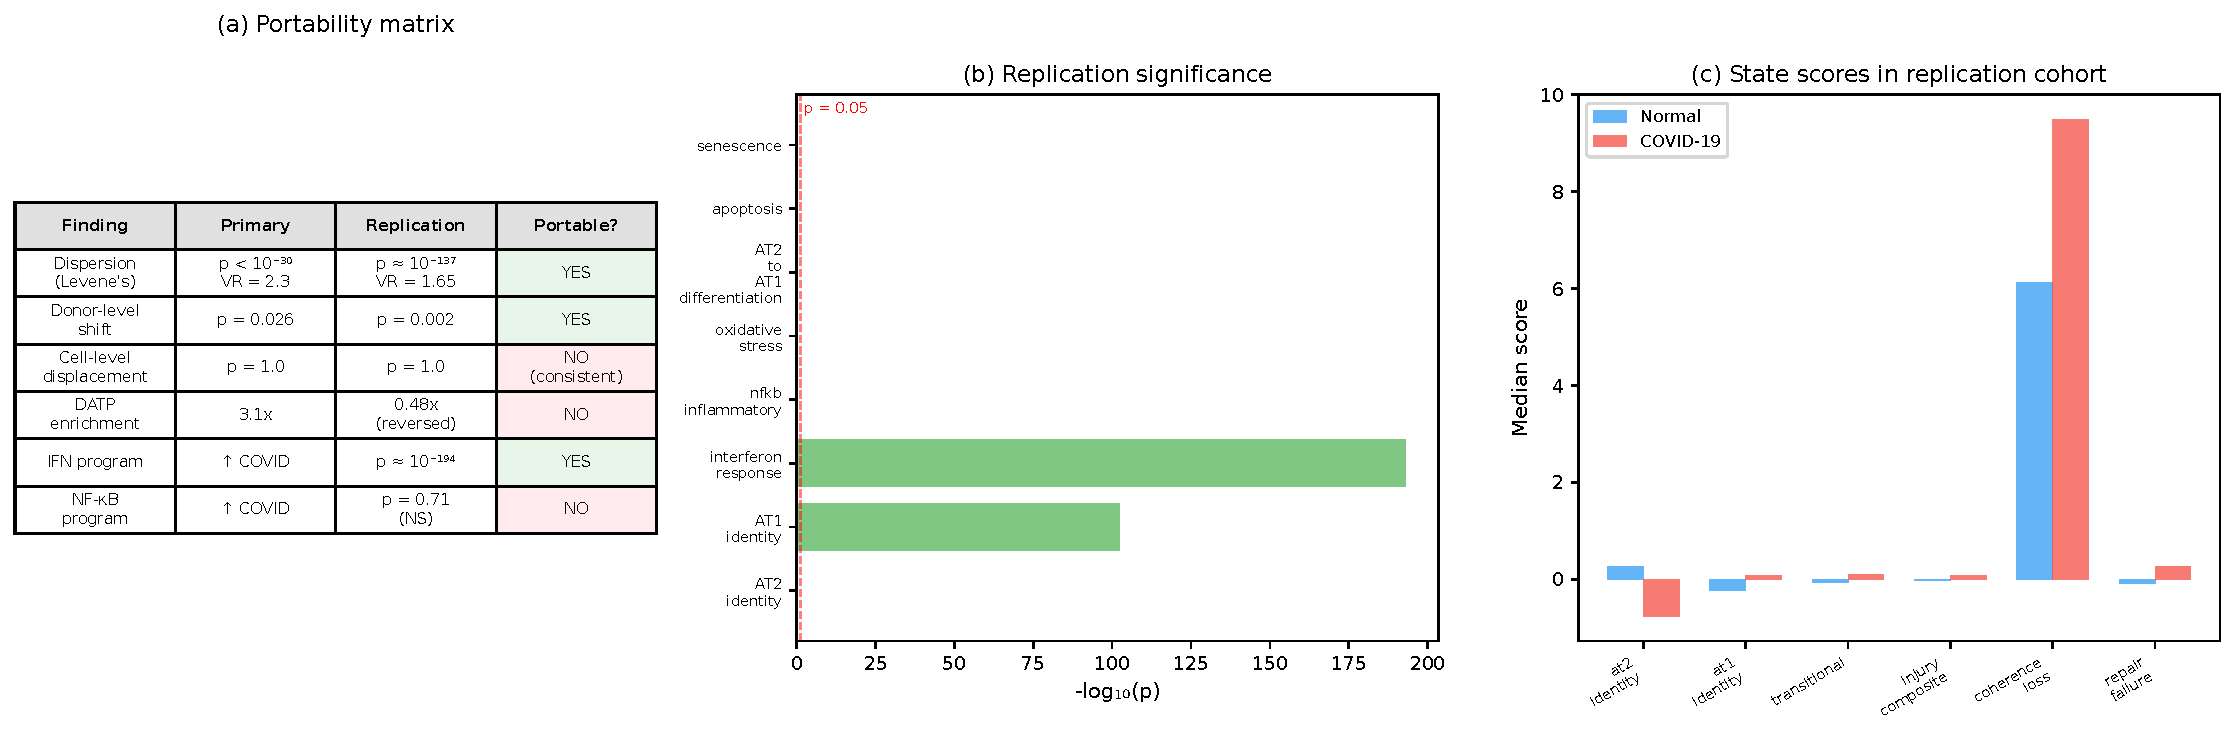
\includegraphics[width=\textwidth]{fig7_replication_summary.pdf}
\caption{Replication summary: portability matrix, per-program significance, and state score distributions.}
\end{figure}


% =========================================================================
\section{Part 8 --- New in v3: donor-level analyses}
% =========================================================================

\begin{vnewbox}
All of Part 8 is new in v3. The key insight: with only 27 donors (7 healthy, 20 COVID), we cannot pretend that 22{,}128 cells are independent observations. Every cell from the same donor shares the same biology. So we need analyses where the donor --- not the cell --- is the unit of inference.
\end{vnewbox}

\subsection{Donor summary statistics}

For each of the 27 donors, we computed:
\begin{itemize}
\item Median pseudotime across all of that donor's cells
\item IQR (interquartile range) of pseudotime
\item Within-donor dispersion: how spread out that donor's cells are in PCA space
\item Fraction of cells annotated as transitional
\item Median score for each of the 8 gene programs
\end{itemize}

\subsection{Donor-level Mann--Whitney tests}

For each metric above, we ran a two-sided Mann--Whitney $U$ test comparing 20 COVID donors against 7 healthy donors. Effect sizes are rank-biserial correlations.

\begin{resultbox}
\textbf{Key result}: Donor-level Mann--Whitney for median pseudotime: $p = 0.026$. This means the donor-level pseudotime shift is significant even when using only 27 data points instead of 22{,}128.
\end{resultbox}

\subsection{Bootstrap confidence intervals}

We resampled \emph{donors} (not cells) with replacement 10{,}000 times within each condition group and computed the difference in group medians at each replicate.

\begin{resultbox}
\textbf{Pseudotime difference}: observed $+0.041$, 95\% CI $[-0.013, +0.086]$. The CI marginally includes zero, reflecting the low power of 7-vs-20 donors. But the cell-level permutation ($p = 0.001$) and cross-cohort replication ($p = 0.002$ at donor level) provide independent corroboration.
\end{resultbox}

\subsection{OLS donor-level regression}

We fit a simple linear regression: $\text{median\_pseudotime} \sim \text{is\_covid}$, with each donor as one observation ($n = 27$).

\begin{resultbox}
\textbf{Result}: COVID coefficient $= +0.043$ (95\% CI $[0.010, 0.076]$; $p = 0.013$; $R^2 = 0.22$). Being a COVID donor is associated with 0.043 units higher median pseudotime, and condition explains 22\% of the donor-level variance in median pseudotime.
\end{resultbox}

\begin{whyblock}
Why OLS and not a mixed-effects model? With exactly one observation per donor, a random intercept for donor is unnecessary --- each donor contributes exactly one row. A random intercept for ``study'' would be appropriate in the replication cohort (multiple studies), but not in the single-study primary cohort.
\end{whyblock}

\subsection{Donor-level dispersion: a surprising result}

\begin{vnewbox}
We computed per-donor within-donor dispersion: for each donor, how spread out are that donor's cells in PCA space? Then we compared per-donor dispersions between conditions.

\textbf{Result}: COVID donors had median dispersion 7.77; healthy donors had 10.58. This is the \emph{opposite} direction from the cell-level finding!

\textbf{Interpretation}: Individual COVID donors are not more internally dispersed than individual healthy donors. The cell-level dispersion signal (Levene $p < 10^{-30}$) arises from \emph{between-donor heterogeneity}: each COVID donor's cells occupy a different region of injury space, and when you pool all COVID cells together, the aggregate looks dispersed. This is actually a more nuanced and biologically interesting finding than uniform within-donor inflation.
\end{vnewbox}


% =========================================================================
\section{Part 9 --- New in v3: portable state scores}
% =========================================================================

\begin{vnewbox}
The DATP marker-threshold approach failed cross-cohort. We need continuous, manifold-based scores that don't depend on arbitrary cutoffs. We developed six:
\end{vnewbox}

\begin{description}[style=nextline]
\item[1. AT2 identity score] Mean expression of 9 AT2 marker genes. Higher = more AT2-like.
\item[2. AT1 identity score] Mean expression of 8 AT1 marker genes. Higher = more AT1-like.
\item[3. Transitional score] Mean expression of 8 transitional markers (KRT8, CLDN4, SFN, etc.). Higher = more transitional.
\item[4. Injury composite] Mean of the six non-homeostatic program scores (interferon, NF-$\kappa$B, oxidative stress, apoptosis, senescence, differentiation). Higher = more injury-program activation.
\item[5. Coherence loss] Euclidean distance from each cell to the centroid of healthy cells in PCA space. Higher = further from healthy identity.
\item[6. Repair failure] Transitional score minus 0.5$\times$(AT2 identity + AT1 identity). High values = cells expressing transitional markers without retaining homeostatic identity. Captures cells that started repair but got stuck.
\end{description}

\subsection{Benchmark results}

\begin{resultbox}
\textbf{Coherence loss} achieved AUC = 0.972 for detecting annotated transitional cells --- nearly perfect, confirming that geometry-based scores capture the transitional phenotype without requiring marker thresholds.
\end{resultbox}

All six scores showed significant condition separation ($p < 10^{-300}$) in the replication cohort, confirming they transfer across cohorts where marker-threshold DATP calling fails.

\begin{figure}[H]\centering
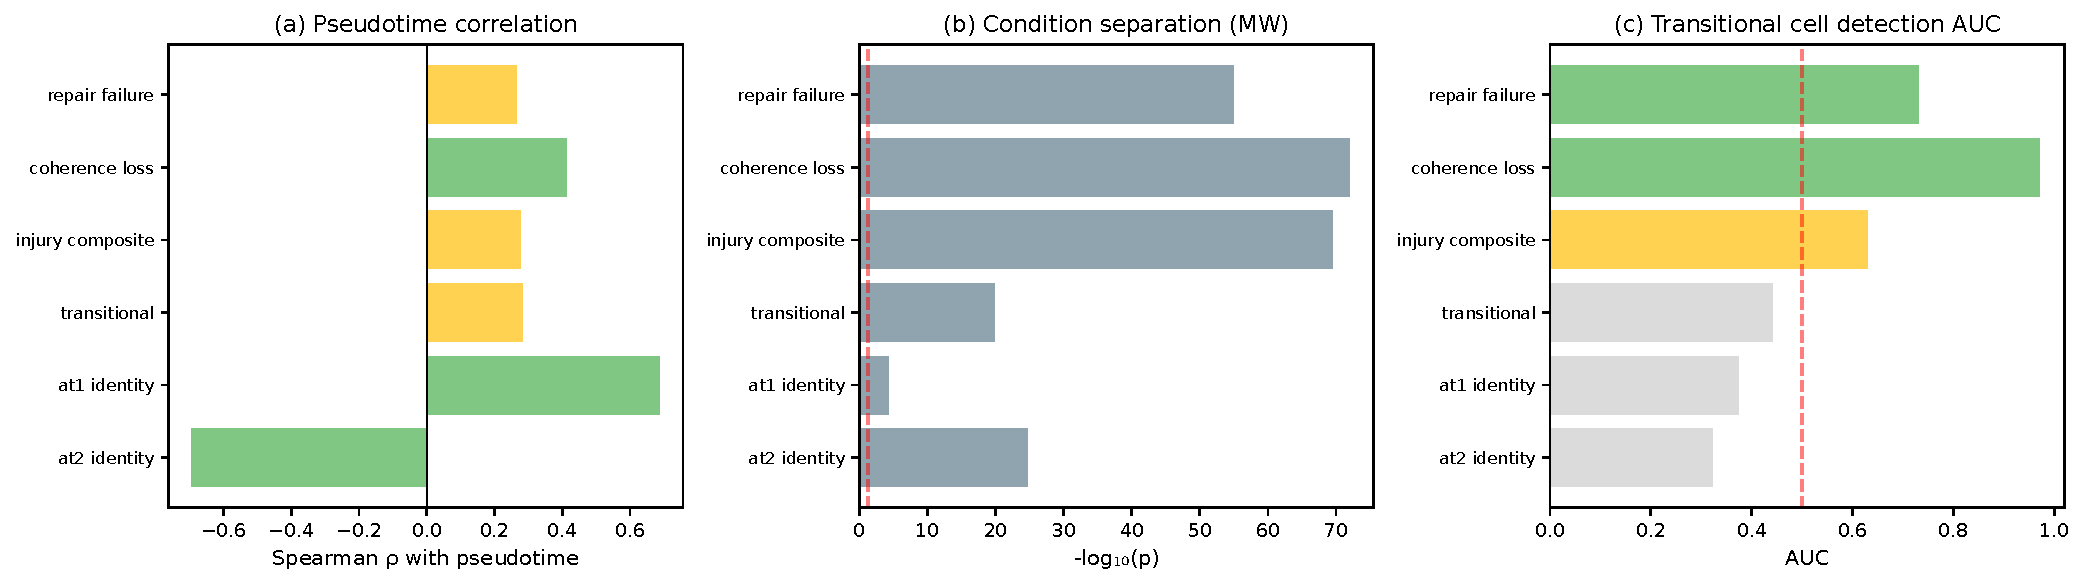
\includegraphics[width=\textwidth]{figS12_state_scores.pdf}
\caption{State score distributions by condition, with benchmark statistics.}
\end{figure}


% =========================================================================
\section{Part 10 --- New in v3: mechanistic decomposition}
% =========================================================================

\begin{vnewbox}
Now that we know the fan-out (dispersion) is the dominant pattern, we can ask: which gene programs contribute most to the fan-out?
\end{vnewbox}

\subsection{Program-geometry linkage}

For each of the 8 gene programs, we computed Spearman correlations with both distance-to-healthy-centroid (``how far from healthy'') and pseudotime (``how far along the trajectory'').

\begin{resultbox}
\textbf{AT2 identity} was the strongest anti-correlate of both distance ($\rho = -0.18$) and pseudotime ($\rho = -0.70$). Cells losing AT2 identity are the ones moving furthest from healthy. \textbf{AT2-to-AT1 differentiation} was the strongest positive correlate of pseudotime ($\rho = 0.31$).
\end{resultbox}

\subsection{Fan-out contribution}

We regressed distance-to-healthy-centroid on all 8 program scores (linear regression, $R^2 = 0.115$):

\begin{center}
\small
\begin{tabular}{lr}
\toprule
Program & Coefficient \\
\midrule
Senescence & $+6.83$ (largest contributor) \\
Oxidative stress & $+3.83$ \\
NF-$\kappa$B inflammatory & $+1.95$ \\
AT2 identity & $-1.13$ \\
AT1 identity & $-1.02$ \\
\bottomrule
\end{tabular}
\end{center}

\begin{resultbox}
The fan-out is driven primarily by divergent activation of stress and senescence programs across cells. Cells retaining homeostatic identity (negative coefficients) are closer to the healthy centroid.
\end{resultbox}

\subsection{Repair-stall analysis}

We computed the ratio of AT2-to-AT1 differentiation score to apoptosis score across pseudotime bins, split by condition. In healthy controls, the differentiation/apoptosis ratio stays higher at late pseudotime. In COVID-19, it drops --- consistent with cells that initiate repair but get diverted toward apoptosis rather than completing AT1 differentiation.

\begin{figure}[H]\centering
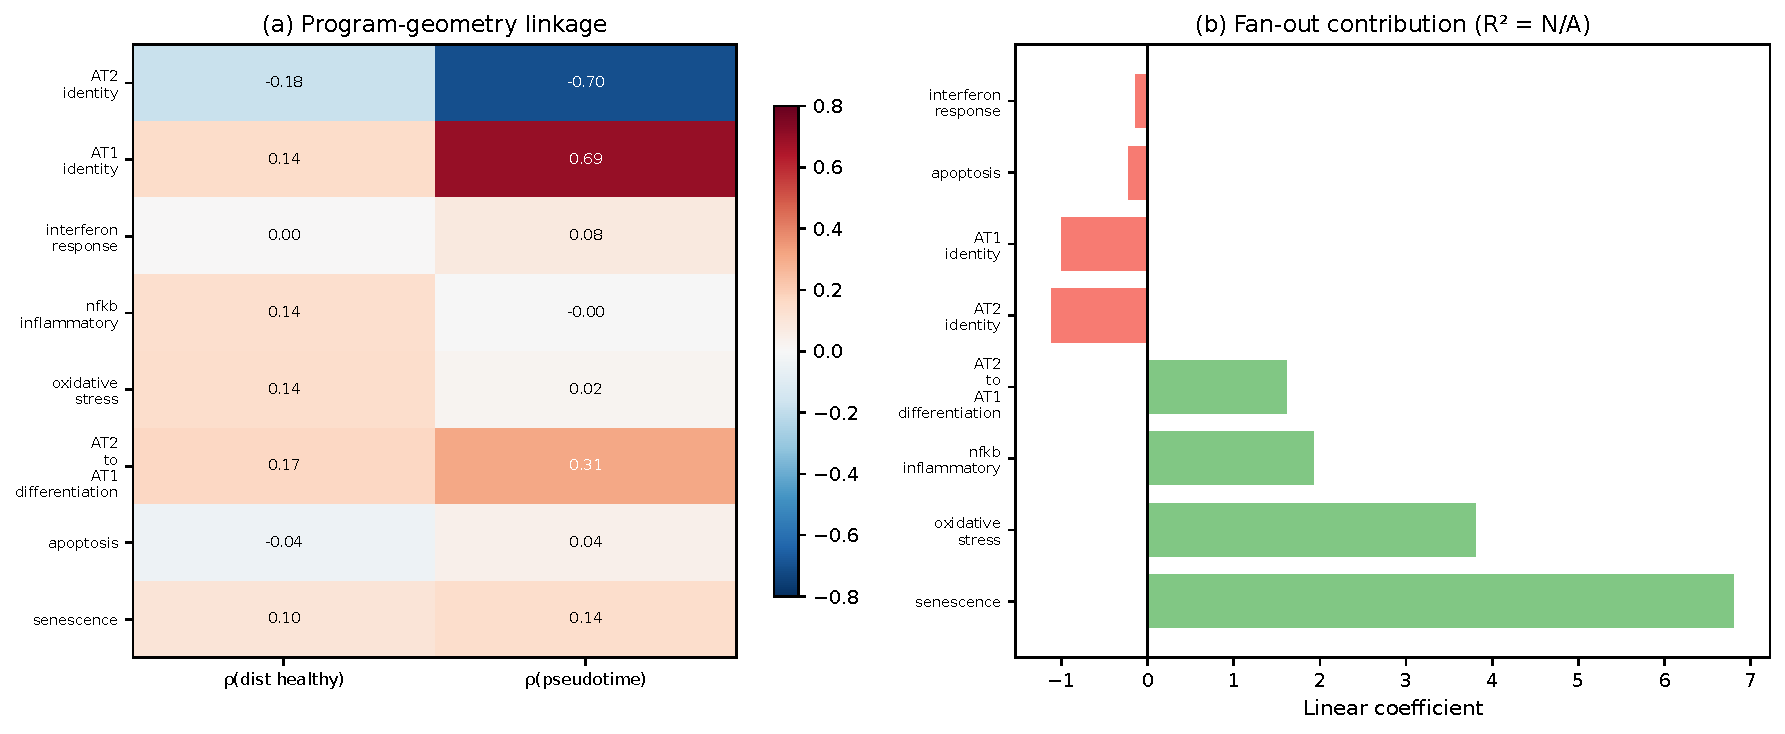
\includegraphics[width=\textwidth]{figS13_mechanism.pdf}
\caption{Mechanistic decomposition. Program-geometry linkage, fan-out regression coefficients, and repair-stall analysis.}
\end{figure}


% =========================================================================
\section{Part 11 --- Reading the main figures}
% =========================================================================

\subsection{Figure 2 --- The manifold (UMAP overview)}

\begin{figure}[H]\centering
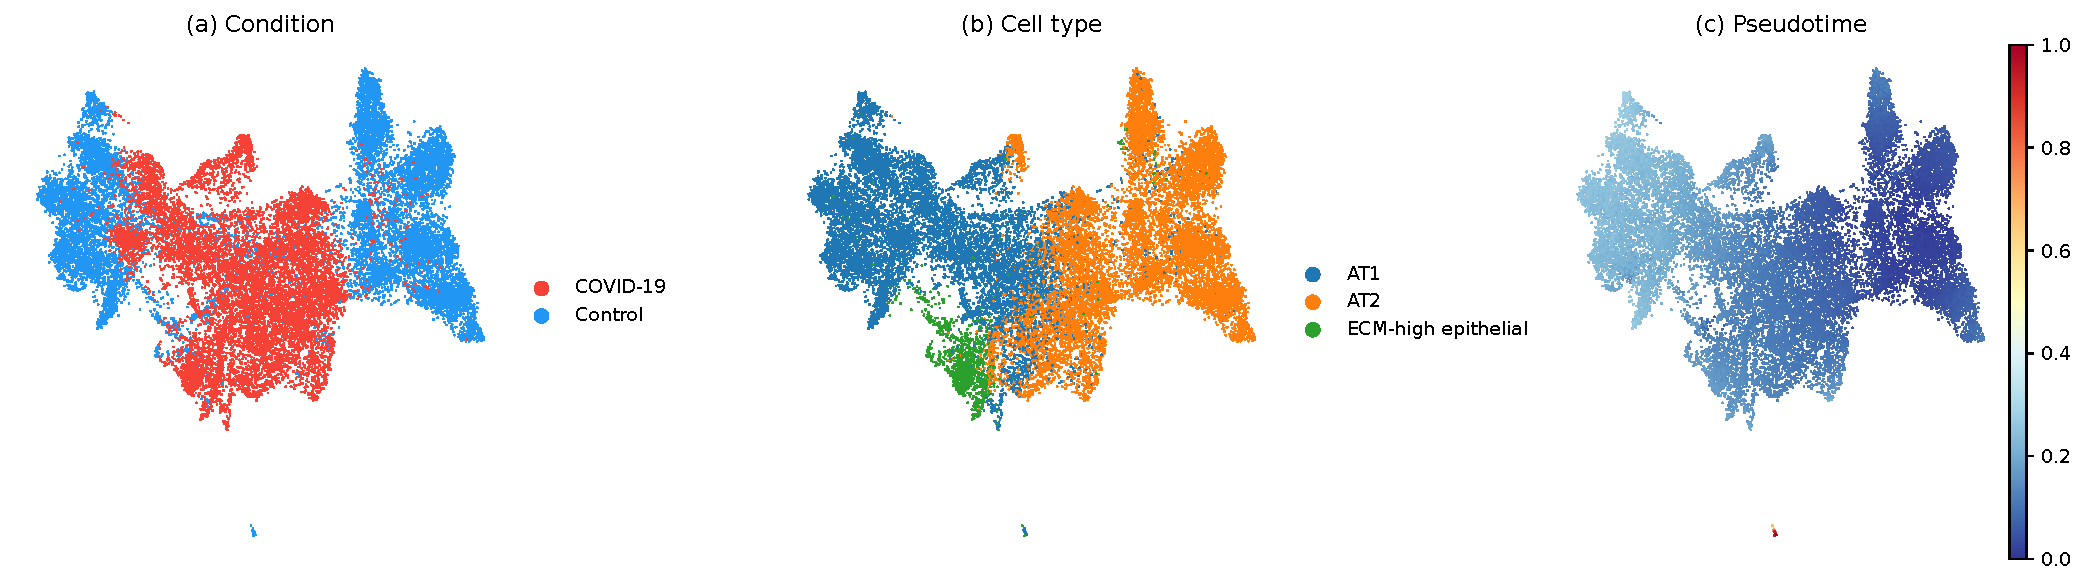
\includegraphics[width=\textwidth]{fig2_manifold.pdf}
\caption{Three-panel UMAP: condition (left), cell type (center), pseudotime (right).}
\end{figure}

\begin{resultbox}
\textbf{How to read it}: If COVID and Healthy cleanly split into different regions, you'd see solid-color blobs. They \emph{overlap}, meaning no mono-directional displacement. The COVID cloud is more spread out. Cell types show the expected structure: AT2 on one side, AT1 on the other, transitional between. Pseudotime grades smoothly from root (healthy AT2) outward.
\end{resultbox}

\subsection{Figure 3 --- Dispersion centerpiece}

See the figure in Part 5, Result 2 above. This is the most important figure in the paper. It shows: (a) within-group distance distributions proving COVID cells are more spread out; (b) displacement test proving centroids are not shifted; (c) donor-level dispersion showing the between-donor heterogeneity mechanism; (d) replication cohort dispersion confirming portability.

\subsection{Figure 5 --- Transitional compartment}

\begin{figure}[H]\centering
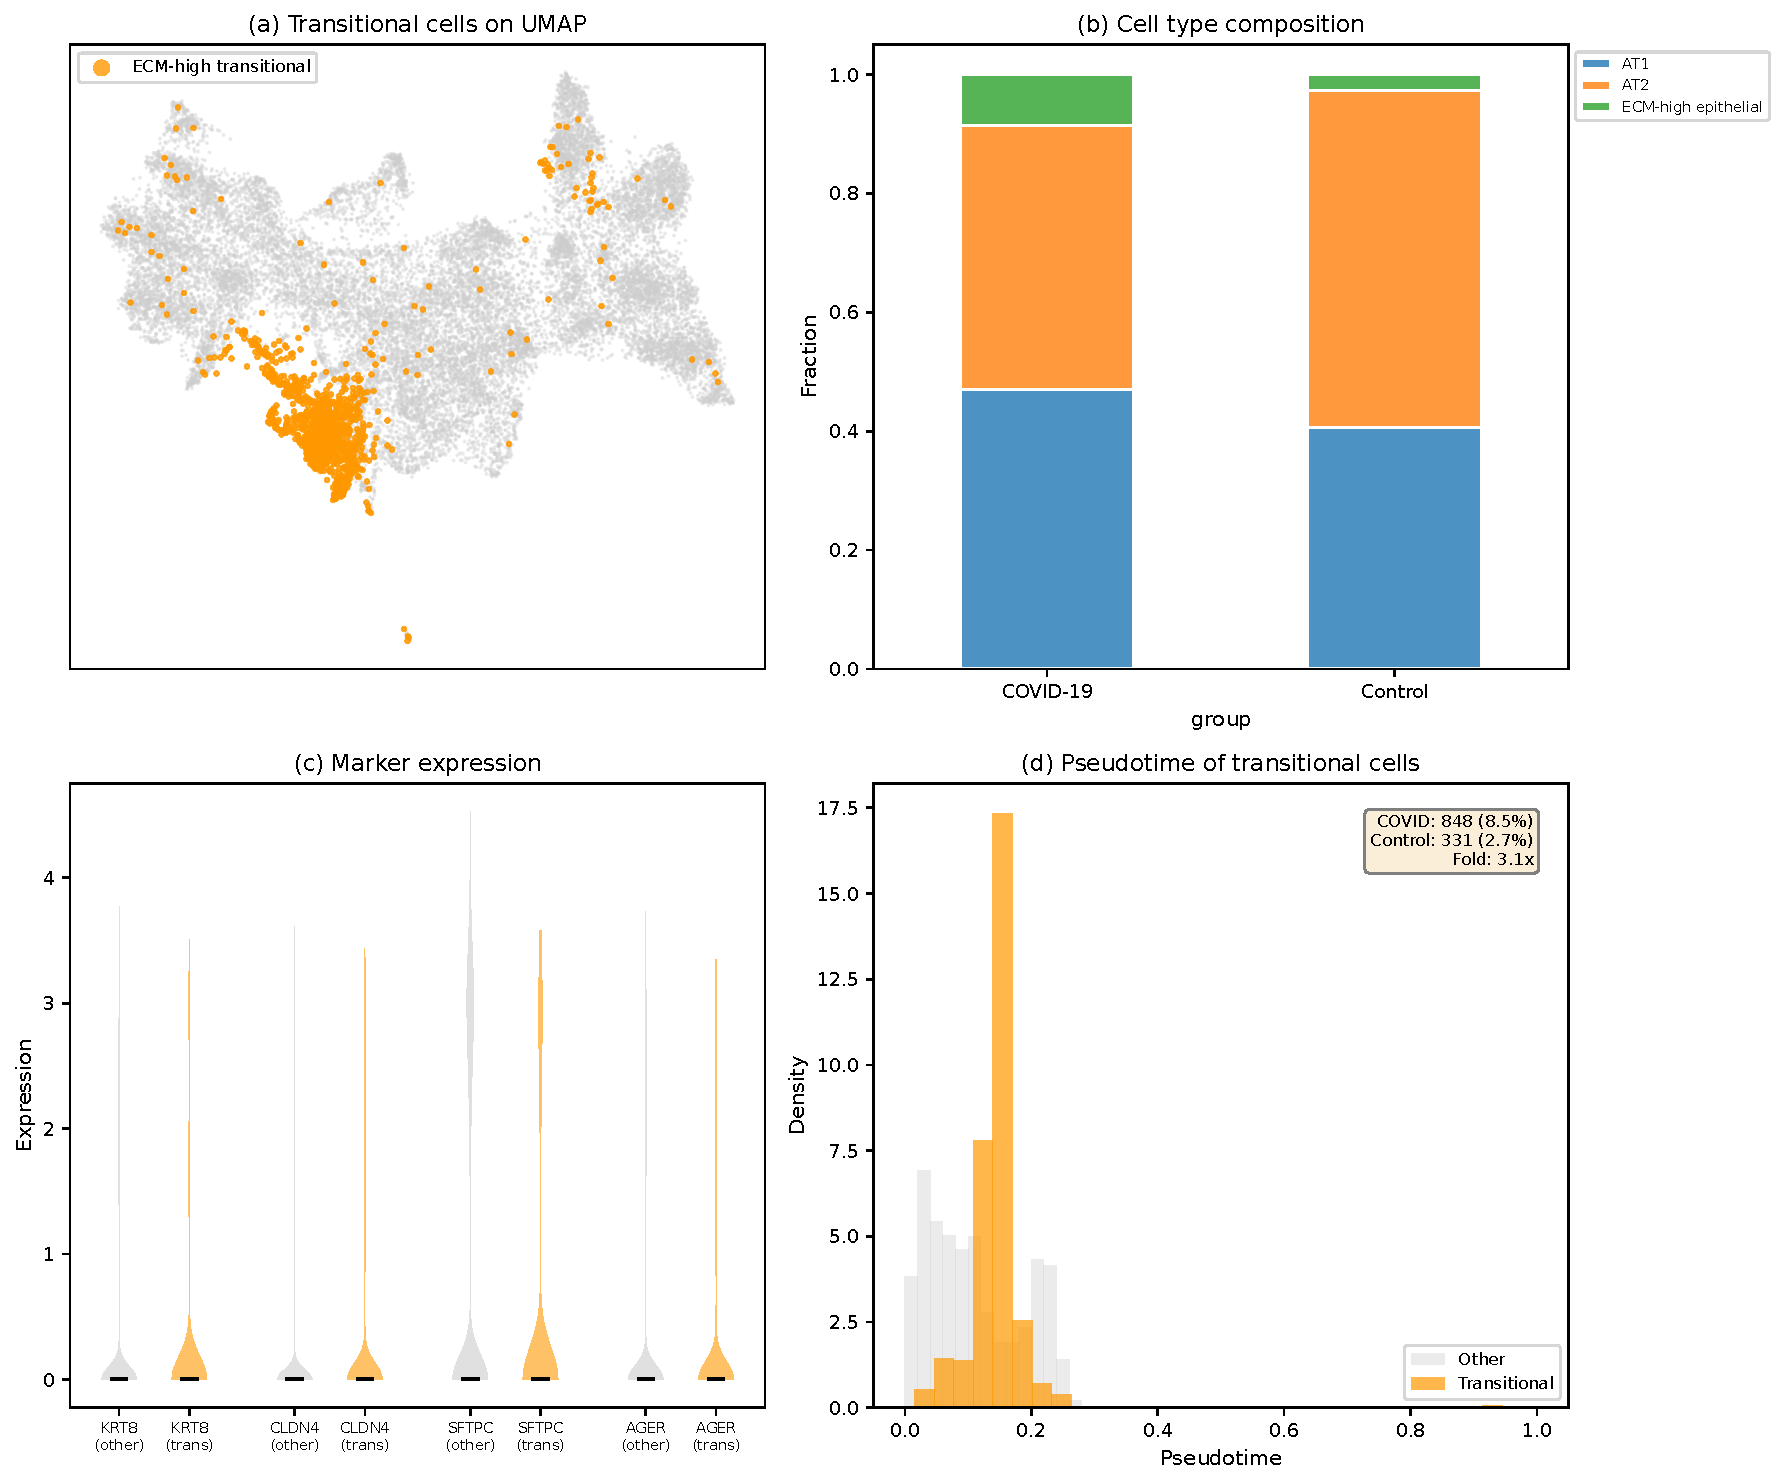
\includegraphics[width=\textwidth]{fig5_transitional.pdf}
\caption{Transitional cell analysis: UMAP highlight, composition bar, markers, pseudotime density.}
\end{figure}

\begin{resultbox}
Transitional cells sit between AT2 and AT1 on the UMAP (intermediate pseudotime), express KRT8/CLDN4, and are 3.1$\times$ enriched in COVID. But remember: this enrichment does not replicate cross-cohort using marker thresholds.
\end{resultbox}


% =========================================================================
\section{Part 12 --- Summary of key tables}
% =========================================================================

\subsection{Table 2: Three pre-registered tests}

\begin{center}
\small
\begin{tabular}{lrrrl}
\toprule
Test & Statistic & $p$-value & Effect size & Outcome \\
\midrule
Displacement (MW) & $5.21 \times 10^7$ & 1.0 & $r = 0.14$ (wrong dir.) & \textbf{Fails} \\
Dispersion (Levene) & 276.5 & $< 10^{-30}$ & ratio 2.3$\times$ & \textbf{Supported} \\
Pseudotime (permutation) & --- & 0.001 & MPD $+0.048$ & \textbf{Supported} \\
\bottomrule
\end{tabular}
\end{center}

\subsection{State score benchmarks}

\begin{center}
\small
\begin{tabular}{lrrrr}
\toprule
Score & $\rho$(pseudotime) & MW $p$ & AUC (transitional) \\
\midrule
AT2 identity & $-0.693$ & $1.7 \times 10^{-25}$ & 0.323 \\
AT1 identity & $+0.687$ & $5.7 \times 10^{-5}$ & 0.375 \\
Transitional & $+0.282$ & $1.3 \times 10^{-20}$ & 0.441 \\
Injury composite & $+0.276$ & $3.8 \times 10^{-70}$ & 0.630 \\
Coherence loss & $+0.412$ & $1.1 \times 10^{-72}$ & \textbf{0.972} \\
Repair failure & $+0.265$ & $1.3 \times 10^{-55}$ & 0.730 \\
\bottomrule
\end{tabular}
\end{center}

\subsection{Donor-level model results}

\begin{center}
\small
\begin{tabular}{lr}
\toprule
Metric & Value \\
\midrule
OLS coefficient (is\_covid) & $+0.043$ \\
OLS $p$-value & 0.013 \\
OLS 95\% CI & $[0.010, 0.076]$ \\
OLS $R^2$ & 0.22 \\
Donor-level MW $p$ & 0.026 \\
Bootstrap 95\% CI for $\Delta$median & $[-0.013, +0.086]$ \\
$n$ donors & 27 \\
\bottomrule
\end{tabular}
\end{center}


% =========================================================================
\section{Part 13 --- How the conclusion was assembled}
% =========================================================================

The conclusion is \textbf{not} ``we found a new COVID effect.'' It is:

\begin{quote}
\emph{Lethal COVID-19 produces dispersion-dominated loss of alveolar epithelial state coherence rather than a coherent directional shift. Cells scatter across heterogeneous injury states while maintaining approximately the same average distance from healthy. The dispersion signal is the strongest, most portable finding --- it replicates across 35 independent datasets and 618 donors. Donor-level trajectory direction also replicates. Cell-level displacement does not. Marker-threshold cell-state definitions are atlas-specific.}
\end{quote}

The reason partial results (2/3 tests succeeding) are more informative than all tests succeeding: the failing test \emph{rules out a specific alternative mechanism}. Having both displacement fail and dispersion succeed tells you the geometry is heterogeneous fan-out, not coherent shift.

\begin{vnewbox}
\textbf{v3 additions to the conclusion}:
\begin{enumerate}
\item The cell-level dispersion arises from between-donor heterogeneity: each COVID donor occupies a different region of injury space, collectively producing the fan-out.
\item Continuous state scores (especially coherence loss, AUC = 0.972) transfer cross-cohort where marker thresholds fail.
\item The fan-out is driven by divergent activation of senescence, oxidative stress, and NF-$\kappa$B programs.
\item Donor-level OLS regression confirms the pseudotime shift at $p = 0.013$ with 22\% variance explained.
\end{enumerate}
\end{vnewbox}


% =========================================================================
\section{Part 14 --- How to reproduce everything}
% =========================================================================

\begin{verbatim}
# Set up environment
cd sb_class_project
python -m venv env && source env/bin/activate
pip install -r requirements.txt

# Primary pipeline
python scripts/run_pipeline.py --step all

# v3 analyses (donor models, state scores, mechanisms)
python scripts/run_v3_analyses.py

# All ten ablations
bash scripts/ablations/rerun_all.sh

# Independent replication
python scripts/replication/fetch_replication.py
python scripts/replication/analyze_replication.py

# Generate all v3 figures
python scripts/generate_v3_figures.py

# Compile paper
cd manuscript
pdflatex paper_v3.tex && pdflatex paper_v3.tex
pdflatex supplementary_methods_v3.tex && pdflatex supplementary_methods_v3.tex
\end{verbatim}


% =========================================================================
\section{Part 15 --- Limitations (honest accounting)}
% =========================================================================

\begin{enumerate}
\item \textbf{Cross-sectional, post-mortem, lethal cases only.} Nothing here tells you about moderate COVID.
\item \textbf{27 donors (7 vs 20)} is a small sample. The bootstrap CI for pseudotime difference marginally includes zero. Cross-cohort replication (618 donors) addresses this partially.
\item \textbf{Pseudotime is ordering, not elapsed time.} No claim about actual hours or stages.
\item \textbf{Replication gene panel too narrow} (84 genes) for a new manifold. Full-transcriptome replication is still missing.
\item \textbf{Fine program ordering is hypothesis-generating only.} It inverts under alternative gene lists (Ablation 8).
\item \textbf{DATP marker-threshold enrichment retracted} as a portable statistic.
\item \textbf{Post-mortem effects.} Peri-mortem hypoxia may influence stress and apoptosis programs.
\item \textbf{Between-donor heterogeneity} could partially reflect post-mortem interval differences, not just disease biology.
\end{enumerate}


% =========================================================================
\section{Part 16 --- What to tell a friend}
% =========================================================================

\textbf{To a biologist:} In lethal COVID-19, alveolar epithelial cells don't all move to one damaged state. They fan out along multiple axes of injury, driven by divergent activation of senescence, oxidative stress, and inflammatory programs. This ``state coherence loss'' signature replicates across 618 donors in 35 independent datasets. Marker-threshold DATP assays don't transfer cross-cohort, but continuous manifold-based scores do.

\textbf{To a computer scientist:} We pre-registered three geometric tests with mutually exclusive mechanistic interpretations, ran ten ablations, fixed a 1-line Harmony bug that changed the effect size 2.6$\times$, replicated in a 618-donor held-out atlas, and added donor-level OLS/bootstrap modeling to address the $n = 27$ problem. The methodological takeaway: dispersion beats centroid displacement for heterogeneous disease states, donor-level pseudobulk beats cell-level tests, and continuous state scores beat marker thresholds for cross-cohort portability.

\textbf{To yourself:} The lung epithelium in lethal COVID doesn't collapse by going somewhere new --- it collapses by spreading out. The cleanest way to see that is variance, not distance. And the spread comes from donors being different from each other, not from individual donors being internally messy.

\end{document}
